% prueba.tex
\documentclass{beamer}
%\usepackage[latin1]{inputenc}
\usepackage[spanish,english]{babel}
\usepackage[utf8]{inputenc}
\usepackage{listings}
\usetheme{Boadilla}
\setbeamertemplate{navigation symbols}{}
\title[Ontologías y EEES]{Uso de ontologías para la implantación del Espacio Europeo de Educación Superior en las titulaciones de grado}
\subtitle[Diseño y aplicación]{Diseño y aplicación}
\author{Daniel Martínez Esteban}
\newcommand{\tutor}{Ángel Herranz Nieva}
\institute[FI-UPM]{
	Facultad de Informática\\
	Universidad Politécnica de Madrid\\
}
\date[Junio 2013]{3 de Junio de 2013}

\selectlanguage{spanish}

\begin{document}
%\lstset{language=protege,basicstyle=\sffamily,columns=flexible,mathescape}
%--- Título -------------------------%
\begin{frame}[plain]
	\begin{center}
		
\includegraphics[scale=0.9]{logofi.png}
	\end{center}
	\titlepage
\end{frame}

%--- Diapositivas -------------------%
\begin{frame}{Índice}
\begin{LARGE}
	\begin{enumerate}
		\item Motivación del trabajo.
		\item Modelización del universo.
		\item Aplicaciones del diseño.
		\item Trabajo a futuro.
	\end{enumerate}
\end{LARGE}
\end{frame}

%--- EEES y ECTS --------------------%
\begin{frame}{Motivación del trabajo}
	\begin{huge}
		Espacio	Europeo de Educación Superior
	\end{huge}
	\begin{Huge}
	\[
		\downdownarrows 
	\]
	\end{Huge}
	\begin{huge}
		European Credit Transfer System
	\end{huge}
\end{frame}

%--- Hojas de cálculo ---------------%
\begin{frame}{Motivación del trabajo}
	Estado anterior:
	\begin{center}
		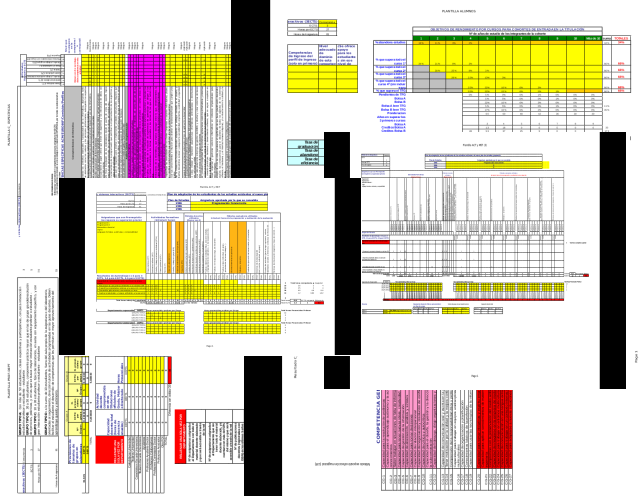
\includegraphics[width=1\textwidth]{collage.png}
	\end{center}
\end{frame}

%--- Unificación, formalización y ---%
%--- procesos automáticos -----------%
\begin{frame}{Motivación del trabajo}
	\begin{LARGE}
		Unificación del conocimiento.
	
		Formalización del conocimiento.
	
		Procesos automatizados
	
	\end{LARGE}
\end{frame}

%--- OWL, ontologías y protegé ------%
\begin{frame}{Modelización del universo}
\begin{LARGE}
	Herramientas utilizadas:
	
	OWL
	\pause	
	
	Ontologías
	\pause
	
	Protegé
	
\end{LARGE}
\end{frame}

%--- Clases y propiedades -----------%
\begin{frame}{Modelización del universo}
\begin{LARGE}

	\begin{itemize}
		\item Clases.
		\item Propiedades.
		\begin{itemize}
			\item Objetos
			\item Tipos de datos
		\end{itemize}
		\item Definiciones
	\end{itemize}		
	
\end{LARGE}
\end{frame}

%--- Diagrama UML de la ontologia ---%
\begin{frame}{Modelización del universo}
	Diagrama UML de la ontología creada:
	\begin{center}
		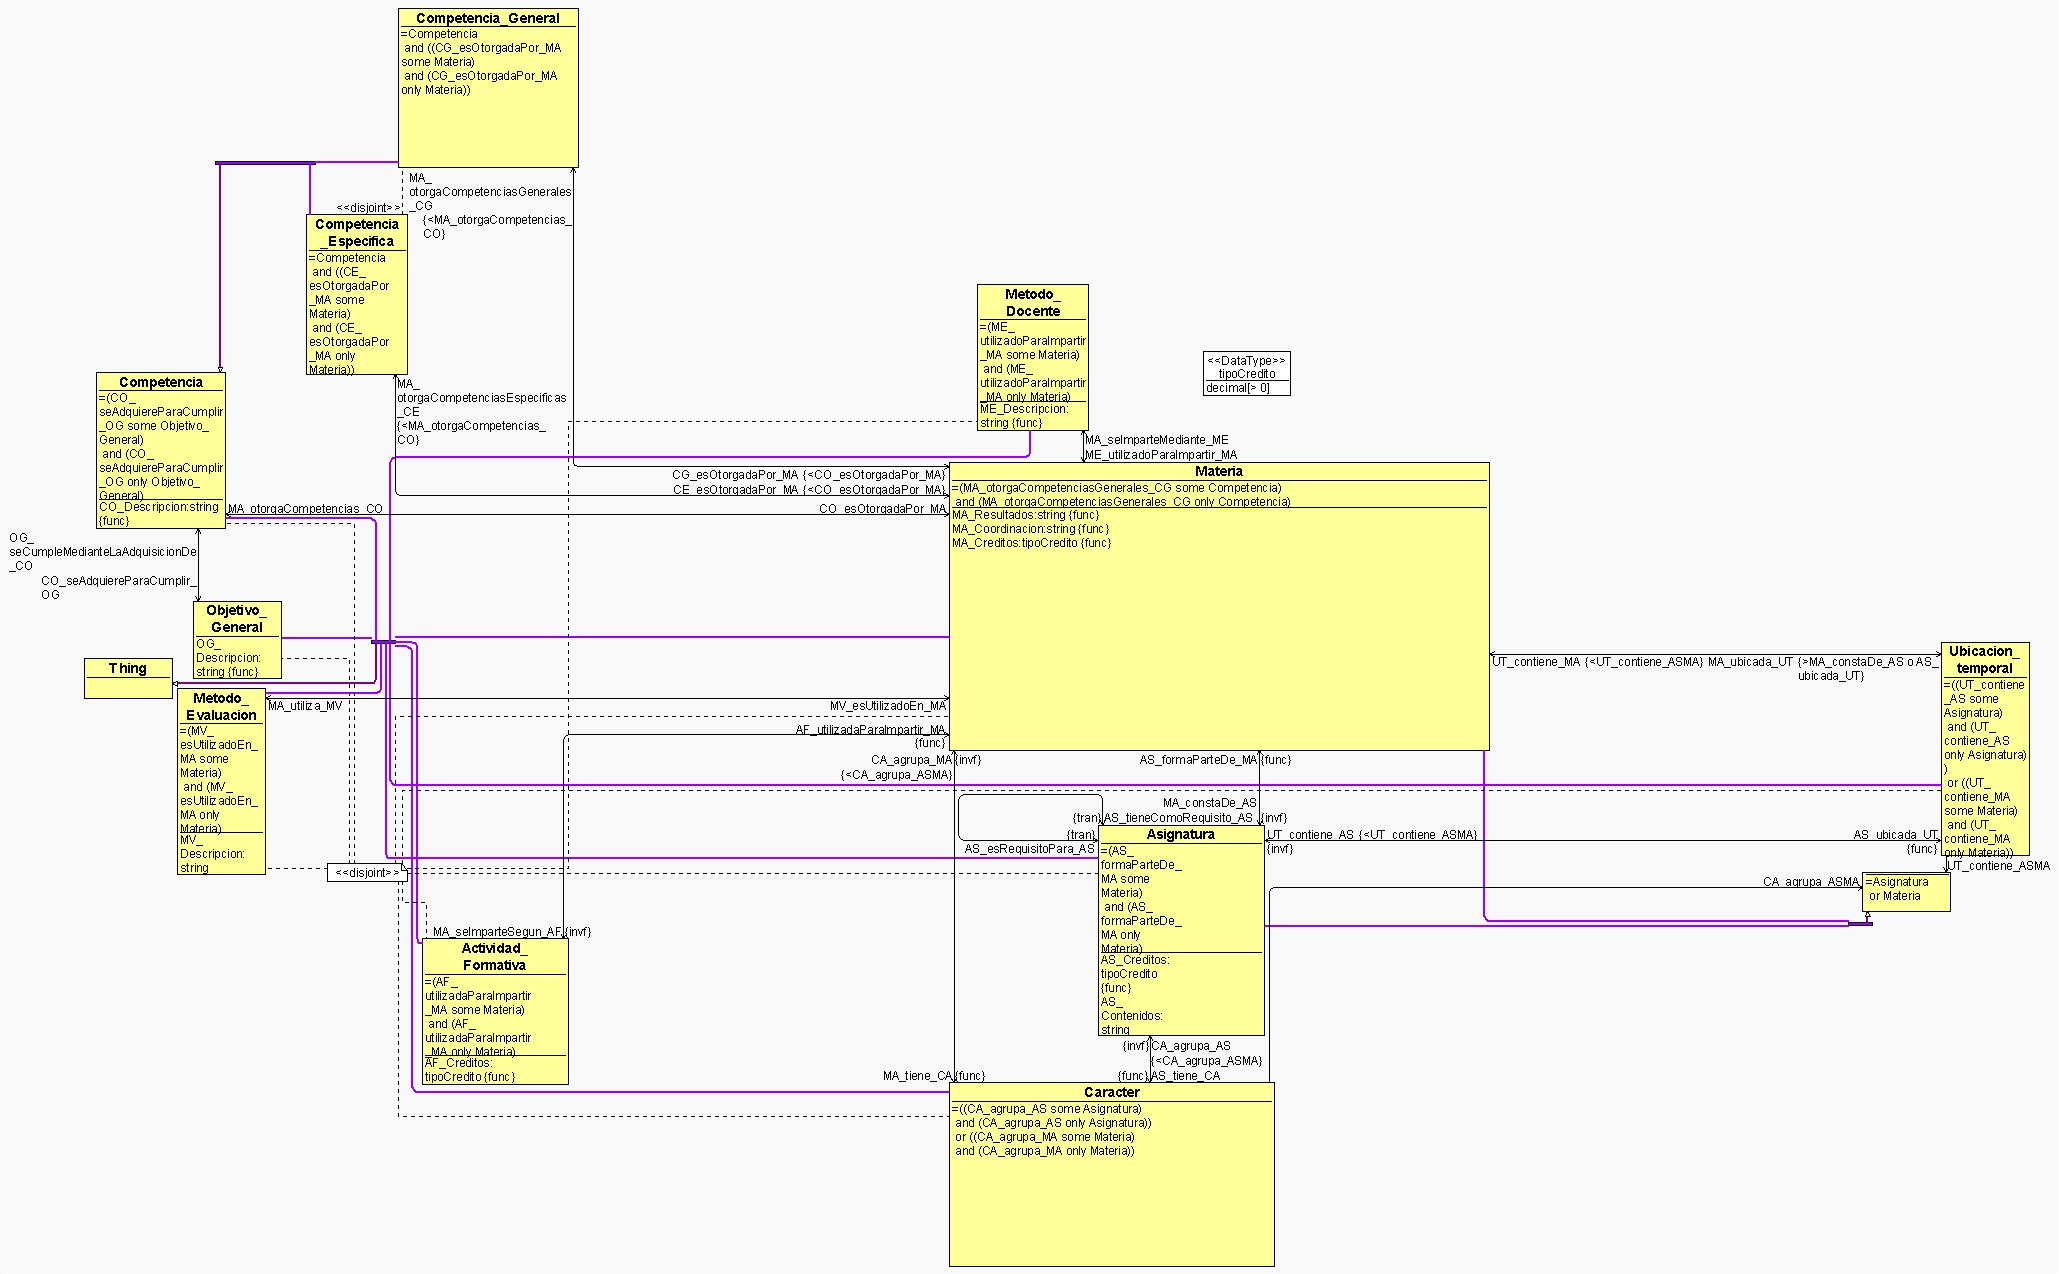
\includegraphics[width=1\textwidth]{Herramientas-OWLGrEd.png}
	\end{center}
\end{frame}

%--- Instancia del plan de estudios -%
\begin{frame}{Aplicaciones del diseño}
%Quiero que aparezca la definición del individuo para que contraste con el batiburillo de las hosjas de cálculo.
%\lstset{language=protege,basicstyle=\sffamily,columns=flexible,mathescape}
%  \lstinputlisting[language=owlms,literate=,linerange=Individual:\ AS\-Concurrencia-xsd:string]{../Texto/a-box.ms} 	
%	\lstinputlisting[linerange={485-498}]{a-box.ms}
%	\begin{center}
%		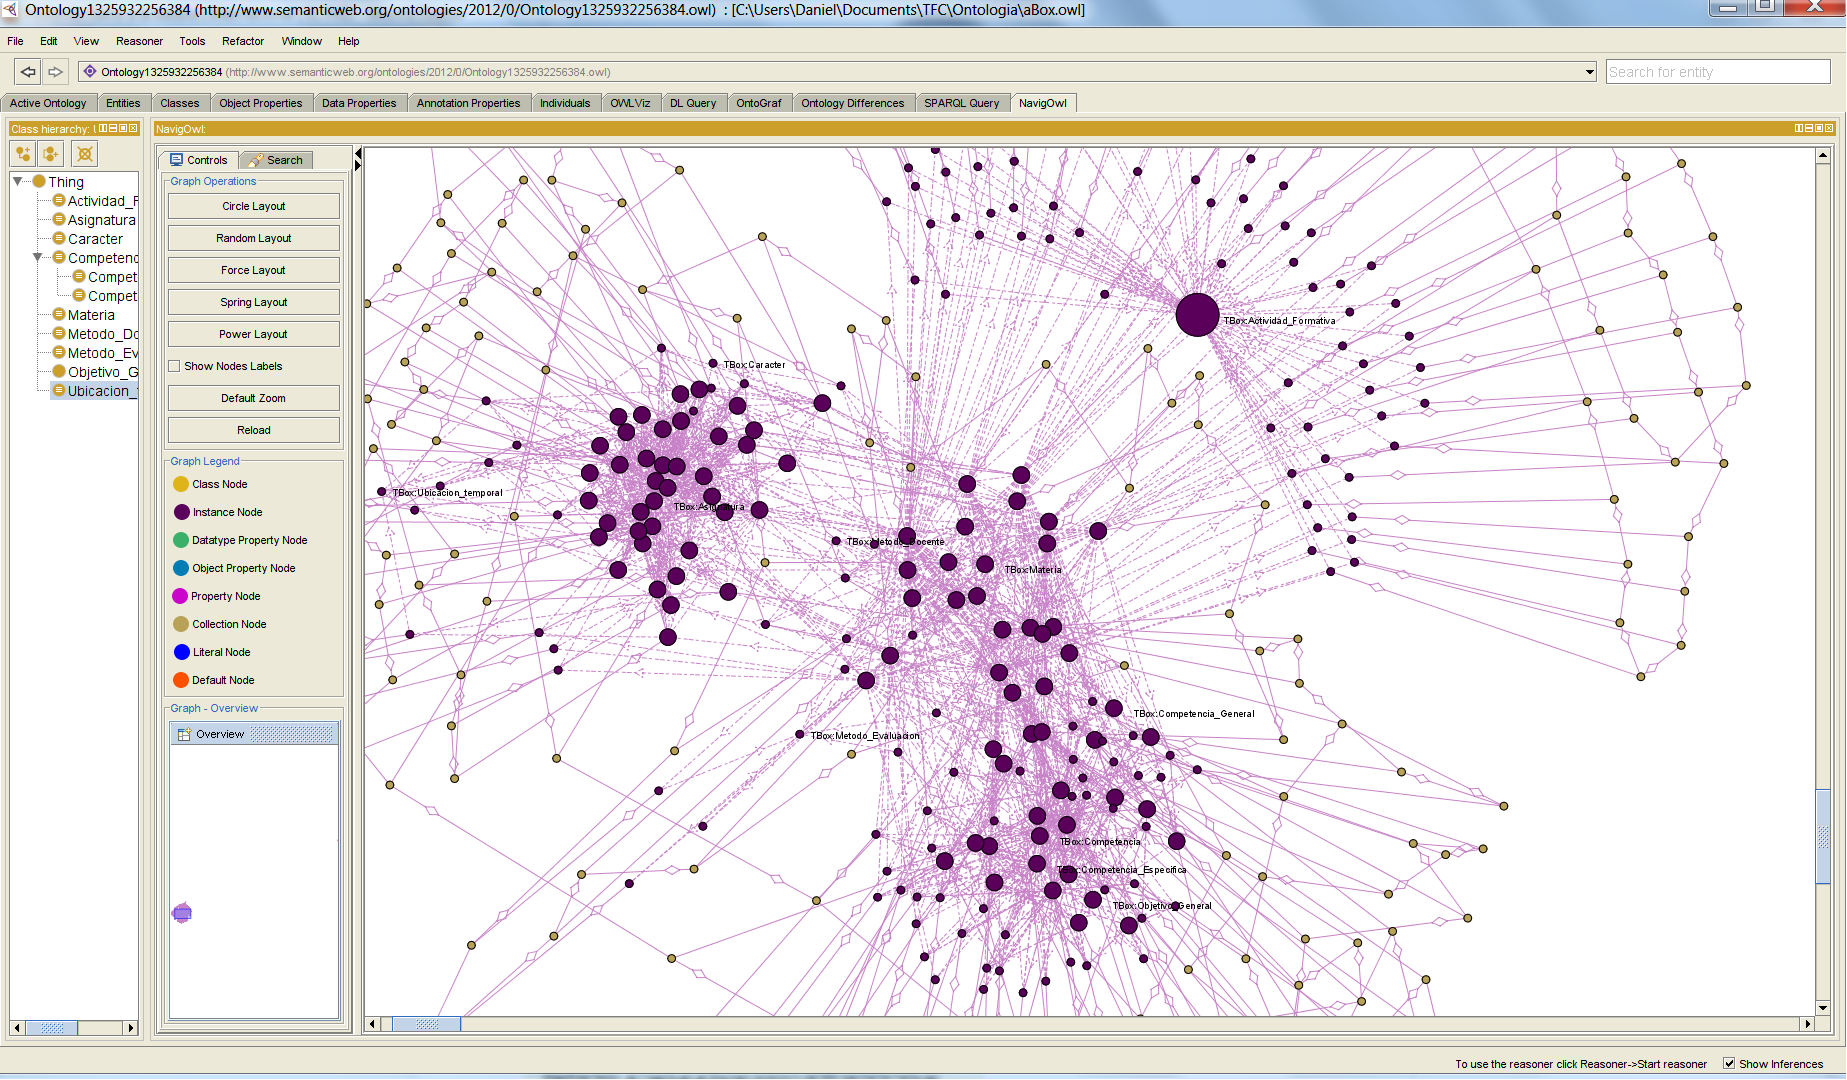
\includegraphics[width=1\textwidth]{Herramientas-NavigOwl.png}
%	\end{center}
	
\end{frame}

\begin{frame}{Aplicaciones del diseño}
\begin{LARGE}
	Aplicaciones automáticas:
	
	Razonadores (FaCT++, HermiT), editores (ACE View, ChangeView, Hypergraph DB), visores (CloudViews, Matrix, NavigOWL, Ontograf, OWLGrEd, SOVA, DL-Query, Cardinality view, Tree views, OWLDoc, OWLViz, OWLPropViz, OWLDiff), transformacion (OWL2RDB).
\end{LARGE}
	
\begin{center}
	{\Huge ¡¡Wiki semántica!!}
\end{center}

\end{frame}

%\begin{frame}{Aplicaciones del diseño}
%	{\Huge ¡Wiki semántica¡}
%\end{frame}

\begin{frame}{Aplicaciones del diseño}
\begin{LARGE}
	Metas alcanzadas:
	\begin{enumerate}
		\item Coherencia con el marco legislativo.
		\item Ayuda al diseño de los itinerarios formativos.
		\item Aplicabilidad por el personal docente.
		\item Seguimiento de los planes docentes.
		\item Orientación al alumno en la elección de centro y estudios.
	\end{enumerate}
\end{LARGE}
\end{frame}

\begin{frame}{Trabajo a futuro}
\begin{LARGE}
	\begin{itemize}
		\item Mejoras en la ontología.
		\item Integración de OWL y Wiki semántica.
		\item Razonadores automáticos sobre la wiki.
	\end{itemize}
\end{LARGE}
\end{frame}

\begin{frame}[c]{}
	\begin{center}
		Gracias por su atención.
	\end{center}
\end{frame}

\end{document}
